\documentclass[beamer]{standalone}%


\begin{document}
\begin{frame}\frametitle{Крива резервів}

  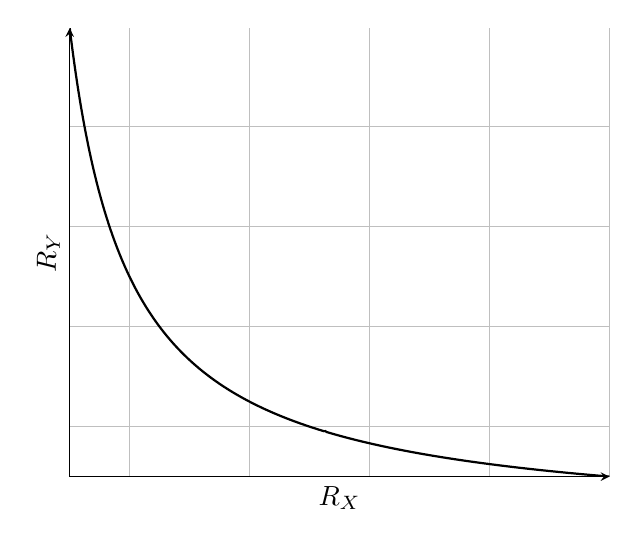
\begin{tikzpicture}[domain=0:4]
    \begin{axis}%
      [
      grid=major,
      ticks=none,
      xlabel={$R_{X}$},
      ylabel={$R_{Y}$},
      axis x line=left,
      axis y line=left,
      no markers,
      domain=0:10,
      restrict y to domain=0:10000
      ]
      \addplot[thick,samples=400] (x,{10000/x});
    \end{axis}
  \end{tikzpicture}
\end{frame}

\begin{frame}\frametitle{Структура біржа на АММ}
  \only<1>{
    \centering
    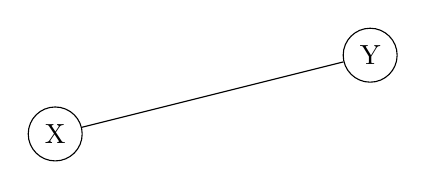
\begin{tikzpicture}
      \node[circle,draw = black] (x) at (0, -1) {X};
      \node[circle,draw = black] (y) at (4, 0) {Y};

      \draw[-] (x) to node [above, sloped] {} (y);
    \end{tikzpicture}
  }
  \only<2>{
    \centering
    \begin{tikzpicture}
      \node[circle,draw = black] (x) at (0, -1) {X};
      \node[circle,draw = black] (y) at (4, 0) {Y};
      \node[circle,draw = black] (z) at (8, 0) {Z};
      \node[circle,draw = black] (w) at (4, -2) {W};

      \draw[-] (x) to node [above, sloped] {} (y);
      \draw[-] (y) to node [above] {} (z);
      \draw[-] (x) to node [below,sloped] {} (w);
    \end{tikzpicture}
  }
  \only<3>{
    \centering
    \begin{tikzpicture}
      \node[circle,draw = black] (x) at (0, -1) {X};
      \node[circle,draw = black] (y) at (4, 0) {Y};
      \node[circle,draw = black] (z) at (8, 0) {Z};
      \node[circle,draw = black] (w) at (4, -2) {W};
      \node[circle,draw = black] (v) at (8, -2) {V};
      \node[circle,draw = black] (u) at (0, -3) {U};
      \node[circle,draw = black] (t) at (4, -4) {T};

      \draw[-] (x) to node [above, sloped] {} (y);
      \draw[-] (y) to node [above] {} (z);
      \draw[-] (x) to node [below,sloped] {} (w);
      \draw[-] (w) to node [below,sloped] {} (v);
      \draw[-] (x) to node [below,sloped] {} (u);
      \draw[-] (u) to node [below,sloped] {} (t);
    \end{tikzpicture}
  }
  \only<4>{
      \centering\includegraphics[scale=0.15]{presentation/images/data.jpg}
  }
\end{frame}

\end{document}
